\section{Derivazione dell'equazione del calore}
Definiamo innanzitutto le variabili in gioco:\\
$t=$ tempo, $x=$ posizione, $u(t,x)=$ temperatura nella posizione $x$ e al tempo $t$.\\
Nel definire il modello si far\`a uso di:
%
\begin{align*}
& r= \mbox{ tasso di calore per unit\`a di massa dall'esterno } \; [r]=\frac{[cal]}{[tempo][massa]}\\
& \rho= \mbox{ densit\`a (lineare) di massa della barra } \; [\rho]=\frac{[massa]}{[lunghezza]}\\
& q= \mbox{ flusso di calore } \; [q]=\frac{[cal]}{[tempo]}\\
& e= \mbox{ energia interna per unit\`a di massa } \; [r]=\frac{[cal]}{[massa]}\\
\end{align*}

Il primo passo nella derivazione dell'equazione del calore consiste nell'applicare la \textit{Legge di Bilancio}:\\
isolata una porzione $[x_0, x_0+h]$ della barra, il tasso di variazione dell'energia interna eguaglia il flusso agli estremi;
nel caso di sorgente, il tasso di variazione del calore erogato sar\`a sommato al flusso agli estremi.
\[
	\underbrace{\frac{d}{dt}\int_{x_0}^{x_0+h} e(t,x)\rho dx}_\text{Variazione dell'energia rispetto al tempo}
	= \overbrace{q(t,x_0)-q(t,x_0 +h)}^\text{Flusso entrante}
	+\underbrace{\int_{x_0}^{x_0+h} r(t,x) \rho dx}_\text{Flusso della sorgente}
\]
Per il Teorema Fondamentale del Calcolo Integrale
\[
	q(t,x_0)-q(t,x_0 +h) = -\int_{x_0}^{x_0+h} q_x(t,x)dx
\]
dove $q_x$ indica $\frac{dq}{dx}$.

Considerando che l'espressione 
\[
	\frac{d}{dt}\int_{x_0}^{x_0+h} e(t,x)\rho dx
	= -\int_{x_0}^{x_0+h} q_x(t,x)dx
	+\int_{x_0}^{x_0+h} r(t,x) \rho dx
\]
deve essere valida per $x_0$ e $x_0+h$ e che, data la continuit\`a dell'energia \`e possibile portare 
la derivata all'interno del segno di integrale, si ottiene la Legge di Bilancio in forma locale
\[
	\frac{\partial}{\partial t} e(t,x)\rho= -\frac{\partial}{\partial x}q(t,x)+\rho r(t,x)
\]

\`E ora necessario applicare le leggi costitutive, che risultano essere delle leggi sperimentali.\\
La prima, che prende il nome di \textit{Legge di Fourier}, indica che il flusso di calore ($q$) \`e direttamente proporzionale
alla derivata spaziale della temperatura secondo la legge
\[
	q= -ku_x
\]
con $u=u(t,x)$ e $k>0$. Il segno negativo indica che si ha il flusso positivo passando dalla zona pi\`u calda a quella pi\`u fredda.
\[
	[k]= \frac{[cal]}{[tempo]}\frac{[lunghezza]}{[grado]}
\]
La seconda lega invece l'energia alla temperatura
\[
	e= c_lu
\]
dove $c_l$ indica il calore specifico ed \`e $>0$
\[
	[c_l]=\frac{[cal]}{[massa][grado]}
\]
Operando la sostituzione si ottiene
\[
	\rho c_l \frac{\partial}{\partial t} u= k \frac{\partial^2}{\partial x^2}u + \rho r
\]
che riordinata
\[
	u_t= \underbracket{D}_{\mathclap{\text{Risposta termica}}} u_{xx}+f
\]
dove $D=k/c_l\rho$ e $f=r/c_l$.
\[
	[D]=\frac{\cancel{[cal]}[lunghezza]}{[tempo]\cancel{[grado]}}\frac{\cancel{[massa]}\cancel{[grado]}}{\cancel{[cal]}}
	\frac{[lunghezza]}{\cancel{[massa]}}=\frac{[lunghezza]^2}{[tempo]}
\]

L'equazione caratteristica risulta quindi essere, considerata l'equazione differenziale omogenea e sostituendo due variabili algebriche alle due variabili derivate
\[
	u_t= Du_{xx} \;\;\; \Rightarrow \;\;\; T=DX^2
\]
Si noti che \`e l'equazione di una parabola.

%%%%%%%%%%%%%%%%%%%%%%%%%%%%%%%%%%%%%%%%%%%%%%%%%%%%%%%%%%%%%%%%%%%%%%%%%%%%%%%%%%%%%%%%%%%%%%%%%%%%%%%%%%%
\section{Problemi ``Ben Posti''}
Si considerino i cosiddetti ``problemi ben posti'', essi saranno del tipo
\[
	\left\{
	\begin{array}{ll}
		u_t=Du_{xx} & x\in\mathbb{R}, \; 0<t<T \\
		u(0,x)=g(x) & \text{Temperatura Iniziale}\\
		u(t,0)=\alpha(t) \; , \; u(t,L)=\beta(t) & \text{Condizioni di Dirichlet agli estremi}\\
		u_x(t,0)=\alpha(t) \; , \; u_x(t,L)=\beta(t) & \text{Condizioni di Neumann agli estremi}
	\end{array}
	\right.
\]
Le condizioni di Dirichlet corrispondono a fissare la temperatura sui capi della sbarra, mentre con Neumann si fissa
il flusso (condizioni di Neumann nulle significano che la barra \`e isolata agli estremi). Non sono state poste condizioni per $t=T$
per la causalit\`a del sistema in esame.

\section{Unicit\`a e dipendenza continua dai dati}
Si inizia con il considerare la temperatura sulla barra
\[
	E(t)= \frac{1}{2}\int_0^L u^2 (t,x) dx
\]
e la si deriva rispetto al tempo
\[
	E'(t)= \frac{1}{2}\int_0^L 2u(t,x)u_t(t,x)dx
\]
Nel passaggio precedente ci si \`e posti nella condizione in cui la derivata della somma equivale alla somma delle derivate.\\
Considerando ora $u_t=Du_{xx}$ si ottiene
\[
	E'(t)= D\int_0^L u(t,x)u_{xx}(t,x)dx
\]
Ora, utilizzando l'integrazione per parti
\[
	D\left[u(t,x)u_x(t,x)\right]_0^L - D\int_0^L 
	\underbrace{u_x(t,x)u_x(t,x)}_{u_x^2(t,x)}dx
\]
Nel caso di condizioni agli estremi nulle si ha $u(t,0)=u(t,L)=0$, perci\`o il termine $D\left[u(t,x)u_x(t,x)\right]_0^L=0$ e quindi
\[
	E'(t)= - D \int_0^L u_x^2(t,x) dx \leq 0
\]
La derivata negativa indica che $E(t)\leq E(0)$, segue che
\[
	\int_0^L u^2(t,x)dx \leq \int_0^L g^2 (x) dx
\]
Perci\`o, considerato il sistema privo di ingressi e quindi l'equazione
omogenea, l'energia non aumenta.\\
Si consideri nuovamente l'equazione $u_t=Du_{xx}$; essa \`e lineare, perci\`o
se $u_1$ e $u_2$ sono soluzioni e $C_1,\; C_2$ costanti, anche $u=C_1u_1+C_2u_2$ \`e soluzione.\\
Se
\[
	\underbracket{
		\begin{array}{l}
			u_1 \text{ \`e soluzione con temperatura iniziale } g_1 \\
			u_2 \text{ \`e soluzione con temperatura iniziale } g_2
		\end{array}
		}_{\Downarrow}
\]
\[
	u_1-u_2 \text{ \`e soluzione con temperatura iniziale } g_1-g_2
\]
e applicato alla disuguaglianza precedente
\[
	\int_0^L \left(u_1(t,x)-u_2(t,x)\right)^2 dx
	\leq
	\int_0^L \left(g_1(x)-g_2(x)\right)^2 dx
\]
che garantisce:\\
{\bf Unicit\`a}: Se $g_1=g_2$ si ottiene
\[
	\int_0^L \underbrace{\left(u_1(t,x)-u_2(t,x)\right)^2}_\text{sempre positivo o nullo} dx
	\leq 0
\]
essendo la somma di quadrati sempre positiva
\[
	\int_0^L \left(u_1(t,x)-u_2(t,x)\right)^2 dx
	= 0
\]
e quindi $u_1(t,x)=u_2(t,x)$
Perci\`o con le stesse condizioni iniziali si ottiene la stessa soluzione.\\
{\bf Dipendenza continua della soluzione dai dati}:\\
Una differenza infinitesima nelle condizioni iniziali comporta una differenza
infinitesima nella soluzione, garantendo la continuit\`a dai dati (non diverge).

\section{Problema di Cauchy globale}
Riprendendo il problema di Dirichlet con condizioni nulle agli estremi
\[
	\left\{
	\begin{array}{l}
		u_t=Du_{xx} \\
		u(0,x)=g(x) \\
		u(t,0)=0, \; u(t,L)=0
	\end{array}
	\right.
\]
Svincoliamo ora la soluzione da $g(x)$ (sar\`a ripreso successivamente)
\[
	\left\{
	\begin{array}{l}
		u_t=Du_{xx} \\
		u(t,0)=0, \; u(t,L)=0
	\end{array}
	\right.
\]
Procediamo poi utilizzando la tecnica della separazione delle variabili.\\
Si consideri $u(t,x)=v(t)w(x)$, perci\`o
\[
	\left\{
	\begin{array}{l}
		v'(t)w(x)=Dv(t)w''(x) \\
		w(0)=w(L)=0
	\end{array}
	\right.
\]
dividendo per $v(t)w(x)$ si ottiene
\[
	\left\{
	\begin{array}{l}
		\displaystyle{\frac{v'(t)}{v(t)}=D\frac{w''(x)}{w(x)} }\\
		w(0)=w(L)=0
	\end{array}
	\right.
\]
Essendo le variabili di integrazione diverse, equivale a dire
\[
	\frac{v'(t)}{v(t)}=K=D\frac{w''(x)}{w(x)}
\]
con $K$ una costante. Perci\`o si posso spezzare in due equazioni
\[
	\left\{
	\begin{array}{l}
		\displaystyle{D w''(x) - Kw(x) = 0 }\\
		w(0)=w(L)=0
	\end{array}
	\right.
	\;\;\;
	\text{ e }
	\;\;\;
	v'(t)=Kv(t)
\]
Procediamo con il risolvere l'equazione differenziale di secondo grado; 
infatti essa imporr\`a dei vincoli su $K$.
\[
	D\lambda^2-K=0
\]
\[
	\lambda^2=\frac{K}{D}
\]
Si distinguono ora i vari casi:
\begin{itemize}
	\item $K>0$
	\item $K=0$
	\item $K<0$
\end{itemize}

{\bf Se $K>0$}:
\[
	\lambda=\pm \sqrt{\frac{K}{D}}
\]
\[
	w(x)= C_1e^{x\sqrt{\frac{K}{D}}} + C_2e^{-x\sqrt{\frac{K}{D}}}
\]
applicando le condizioni al contorno ($w(0)=0 \; w(L)=0$)
\[
	\left\{
	\begin{array}{l}
		C_1+C_2=0 \\
		\displaystyle{C_1e^{L\sqrt{\frac{K}{D}}} 
			+ C_2e^{-L\sqrt{\frac{K}{D}}}}
	\end{array}
	\right.
	\;\;\;
	\Rightarrow
	\;\;\;
	\left\{
	\begin{array}{l}
		C_1=0\\
		C_2=0
	\end{array}
	\right.
\]
Perci\`o l'insieme delle soluzioni con $K>0$ verr\`a scartato.

{\bf Se $K=0$}:
\[
	w''=0
	\;\;\;
	\Rightarrow
	\;\;\;
	w(x)=C_1x + C_2
\]
\[
	\left\{
	\begin{array}{l}
		w(x)=C_1x + C_2\\
		w(0)=0, \; w(L)=0
	\end{array}
	\right.
	\;\;\;
	\Rightarrow
	\;\;\;
	\left\{
	\begin{array}{l}
		C_1=0\\
		C_2=0
	\end{array}
	\right.
\]
Anche la soluzione con $K=0$ sar\`a scartata.

{\bf Se $K<0$}:\\
Poniamo $-\omega^2 = K/D$ $\Rightarrow$ $\lambda^2 = - \omega^2$ e $\lambda=\pm i\omega$
\[
	\left\{
	\begin{array}{l}
		w(x)=C_1 cos(\omega x) + C_2 sin(\omega x)\\
		w(0)=0, \; w(L)=0
	\end{array}
	\right.
	\;\;\;
	\Rightarrow
	\;\;\;
	\left\{
	\begin{array}{l}
		C_1=0\\
		C_2 sin(\omega L)= 0
	\end{array}
	\right.
\]
\[
	\sin (\omega L)=0
	\;\;\;
	\Rightarrow
	\;\;\;
	\omega L = n\pi
	\;\;\;
	\Rightarrow
	\;\;\;
	\omega_n= \omega= n \frac{\pi}{L} \text{, con }n=1,2,3,\ldots
\]
Ora, considerata la soluzione n-esima di $w(x)$
\[
	w_n(x)=sin\left(\frac{n\pi}{L}x \right)
\]
dove la costante $C_2$ sar\`a considerata successivamente, al momento della scomposizione con Fourier.\\
Considerato ora
\[
	K_n=-\omega_n^2 D= -\left(\frac{n\pi}{L}\right)^2D
\]
procediamo con il risolvere l'equazione differenziale di primo grado
\[
	v'(t)= Kv(t)
\]
\[
	v_n(t)= e^{Kt}=e^{-\left(\frac{n\pi}{L}\right)^2Dt}
\]
Riprendendo  $u_n(t,x)= w_n(x) v_n(t)$ si ottengono le infinite soluzioni
di base del problema di Dirichlet iniziale
\[
	u_n(t,x)= e^{-\frac{n^2\pi^2}{L^2} Dt}
	sin\left(\frac{n\pi}{L}x \right)
\]
A questo punto Fourier considera la possibilit\`a di scomporre qualsiasi
soluzione come serie di sinusoidi, quindi
\[
	u= \sum_{n=1}^{\infty} b_n u_n(t,n)=
	\sum_{n=1}^{\infty}b_n e^{-\frac{n^2\pi^2}{L^2} Dt}
	sin\left(\frac{n\pi}{L}x \right)
\]
dove i vari $b_n$ rappresenterebbero i precedenti $C_{2(n)}$.\\
A questo punto \`e possibile definire anche le condizioni con $t=0$ attraverso
la scomposizione in \texttt{serie di Fourier}, infatti $u(0,x)=g(x)$, perci\`o
\[
	g(x)= \sum_{n=1}^{\infty} b_n sin\left(\frac{n\pi}{L}x \right)
\]
con $0\leq x \leq L$.\\
Bisogna quindi trovare un modo per poter esprimere la funzione $g(x)$
come serie di sinusoidi.\\
Verifichiamo prima di tutto la convergenza.\\
Si prenda una sequenza limitata dei coefficienti $b_n$, cio\`e che
$|b_n|\leq C$ per qualsiasi $n$, data $C$ una costante. Allora se $t \geq t_0 > 0$
e $0\leq x \leq L$
\[
	\sum_{n=1}^{\infty}\left| b_n e^{-\frac{n^2\pi^2}{L^2} Dt}
	sin\left(\frac{n\pi}{L}x \right)\right|
	\leq
	\sum_{n=1}^{\infty}\left| b_n \right| e^{-\frac{n^2\pi^2}{L^2} Dt}
	\leq
	C \underbrace{\sum_{n=1}^{\infty}e^{-\frac{n^2\pi^2}{L^2} Dt}}
	_\text{Serie convergente}
\]
Siccome ogni addendo \`e soluzione dell'equazione, se risulta possibile
derivare all'interno della serie, anch'essa \`e soluzione. Questo pu\`o essere
effettuato nel caso in cui la somma della serie converga.
\[
	\sum_{n=1}^{\infty}\left| \frac{\partial}{\partial x} u_n \right|=
	\sum_{n=1}^{\infty}\left| b_n \frac{n\pi}{L} 
	e^{-\frac{n^2\pi^2}{L^2} Dt}
	sin\left(\frac{n\pi}{L}x \right)\right|
	\leq
	C \sum_{n=1}^{\infty} \frac{n\pi}{L} e^{-\frac{n^2\pi^2}{L^2} Dt}
\]
In questo caso $e^{-n^2}$ tende a zero molto rapidamente, rendendo la serie convergente. Successivamente anche la derivata seconda converge 
(in realt\`a \`e una funzione liscia, cio\`e $u(t,x)\in C^\infty$,
per $t>0$ e $0\leq x \leq L$).
Qualunque sia $g(x)$, passato l'istante $t=0$, la funzione diventa immediatamente
continua. La diffusione ha quindi un effetto regolarizzante.\\
\`E quindi possibile derivare all'interno della sommatoria.\\
Si tratta ora di costruire il prolungamento dispari con periodo $2L$ (fig. \ref{prolper_disp})
\begin{figure}[H]
	\centering
	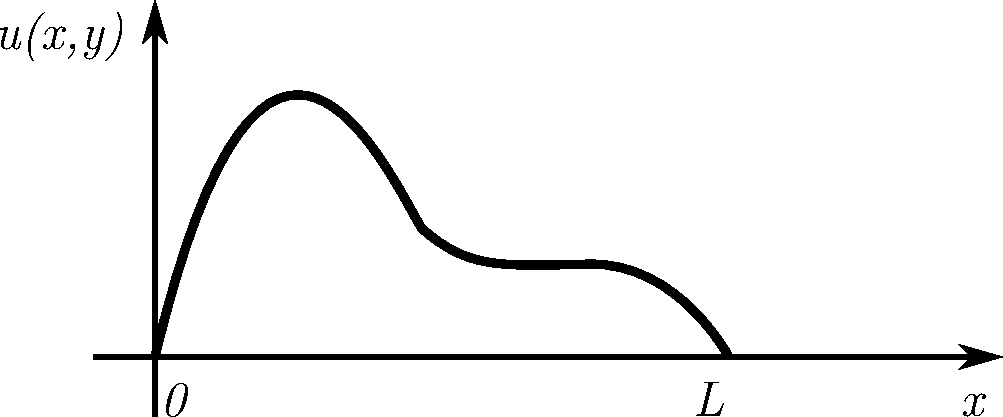
\includegraphics[width=0.5\textwidth]{gx.pdf}
	\caption{Funzione $g(x)$}
	\label{gx}
\end{figure}
\begin{figure}[H]
	\centering
	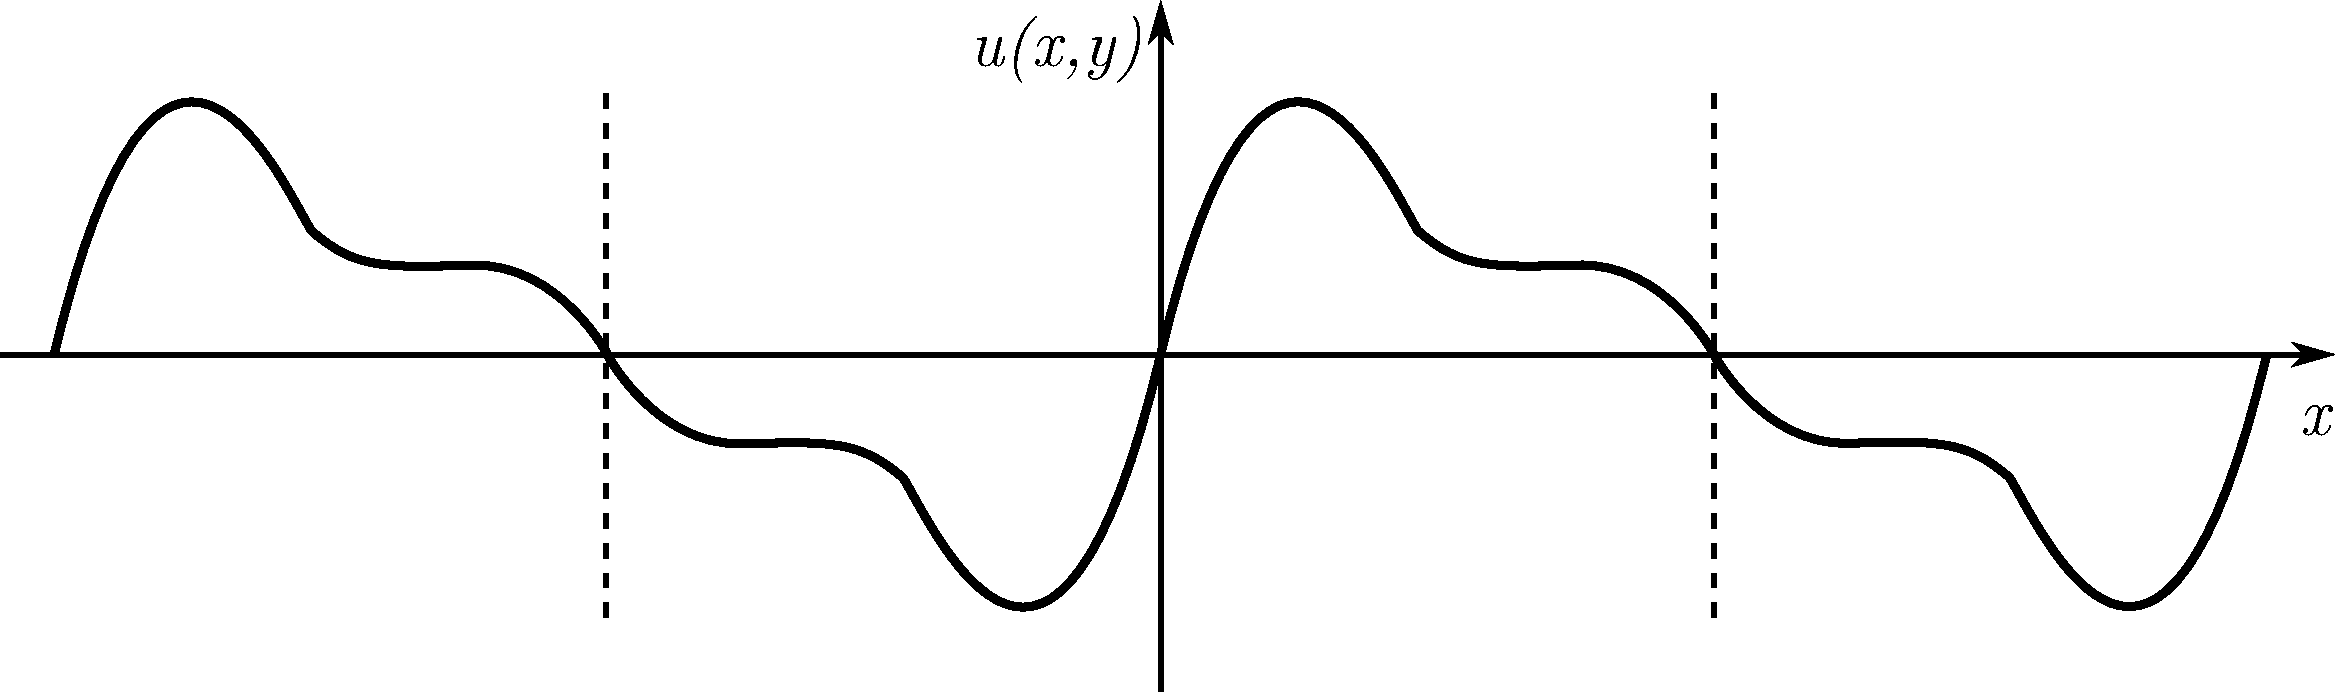
\includegraphics[width=\textwidth]{prolper_disp.pdf}
	\caption{Prolungamento periodico dispari}
	\label{prolper_disp}
\end{figure}
\noindent
Si \`e operato con un prolungamento dispari in modo da ottenere una serie composta
da sole sinusoidi. Si noti che nella parte di interesse, cio\`e tra $0$ e $L$, 
rappresenta effettivamente la funzione $g(x)$.
\[
	b_n= \frac{2}{L}\int_0^L g(x)sin \left(\frac{n\pi}{l} x\right) dx
	\;\;\; \text{con} \;\;\;
	\omega= \frac{2\pi}{2L}= \frac{\pi}{L}
\]
Ricavati i $b_n$ \`e possibile ottenere la funzione $u(x,t)$.

Il coefficiente di scala \`e dato da $D/L^2$; questo consente di 
scalare le dimensioni variando opportunamente il materiale, rendendo possibile
l'uso di modellini equivalenti (scalati).
\[
	\frac{D_1}{L_1^2}= \frac{D_2}{L_2^2}
\]
\subsection{Esercizio: Condizioni agli estremi non nulle}
\[
	\left\{
	\begin{array}{l}
		u_t=Du_{xx} \\
		u(0,x)=g(x) \\
		u(t,0)=\theta_1 \\
		u(t,L)=\theta_2
	\end{array}
	\right.
\]
con $\theta_1 \neq \theta_2$.\\
Si inizia con il considerare una soluzione stazionaria del problema, cio\`e
indipendente dal tempo
\[
	\left\{
	\begin{array}{l}
		\cancel{u_t}=Du_{xx}^S \\
		u(0,x)=g(x) \\
		u^S(\cancel{t},0)=\theta_1 \\
		u^S(\cancel{t},L)=\theta_2
	\end{array}
	\right.
	\;\;\;
	\Rightarrow
	\;\;\;
	\left\{
	\begin{array}{l}
		Du_{xx}^S= 0 \\
		u(0,x)=g(x) \\
		u^S(0)=\theta_1 \\
		u^S(L)=\theta_2
	\end{array}
	\right.
\]
\[
	(u^S)''(x)=0 \;\;\; \Rightarrow \;\;\; u^S(x)=ax+b
\]
\[
	u^S(0)= \theta_1 \;\;\; \Rightarrow \;\;\; b= \theta_1
\]
\[
	u^S(L)= \theta_2 \;\;\; \Rightarrow \;\;\; aL+\theta_1= \theta_2
	\;\;\; \Rightarrow \; \; \; a= \frac{\theta_2 - \theta_1}{L}
\]
\begin{figure}[H]
	\centering
	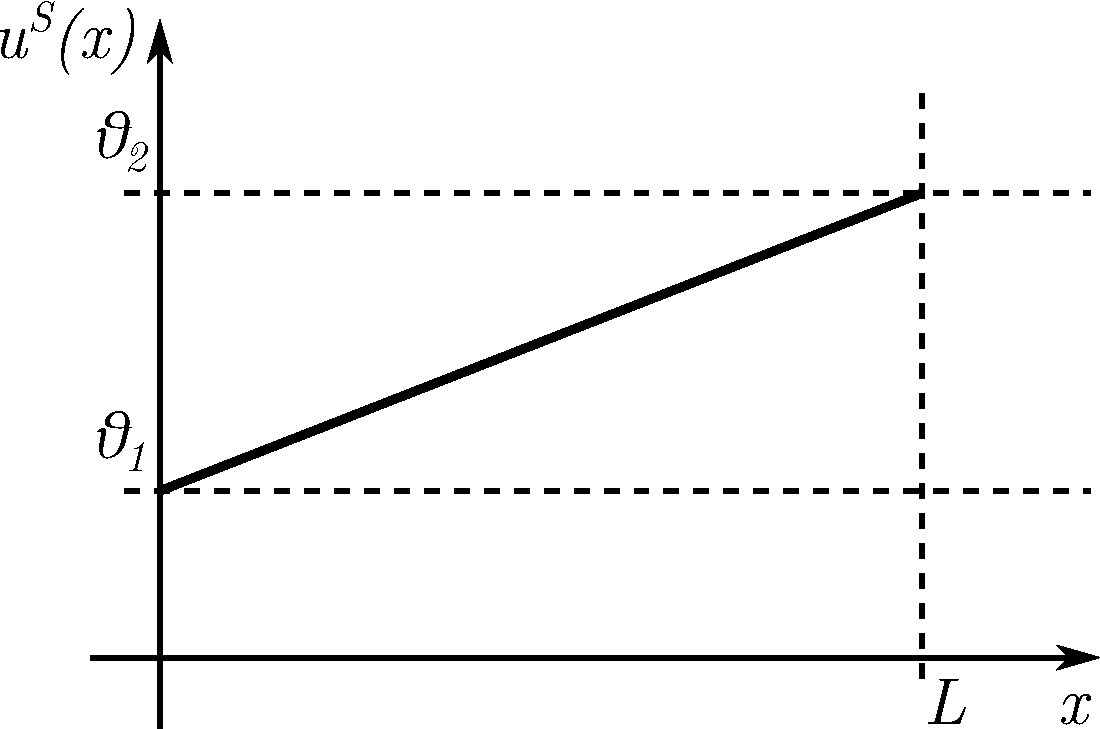
\includegraphics[width=0.5\textwidth]{nonomog_stationary.pdf}
	\caption{Soluzione stazionaria}
	\label{nonomog_stationary}
\end{figure}
La soluzione \`e composta quindi dalla soluzione stazionaria e dalla soluzione
con condizioni agli estremi nulle.
\[
	u(t,x)= \underbrace{v(t,x)}_{\mathclap{\text{Transitorio}}} + u^S(x)
\]
con $u(0,x)= v(0,x) + u^S(x) \;\;\; \Rightarrow \;\;\; v(0,x)=g(x)- u^S(x)$
\[
	\left\{
	\begin{array}{l}
		v_t=Dv_{xx} \\
		v(0,x)=g(x)- u^S(x) \\
		v(t,0)=0 \\
		v(t,L)=0
	\end{array}
	\right.
\] 
\subsection{Esercizio: Barra isolata agli estremi}
\[
	\left\{
	\begin{array}{l}
		u_t=Du_{xx} \\
		u(0,x)=g(x) \\
		u_x(t,0)=0 \\
		u_x(t,L)=0
	\end{array}
	\right.
\]
Si ottiene che la soluzione \`e composta da una serie di soli coseni a 
valor medio non nullo
\[
	u(t,x)= \frac{a_0}{2}+ \sum_{n=1}^\infty a_n 
	e^{-\frac{n^2\pi^2}{L^2} Dt}
	cos \left(\frac{n\pi}{L}x \right)
\]
\[
	\frac{a_0}{2}= \frac{1}{L}\int_0^L g(x)dx
\]
\begin{figure}[H]
	\centering
	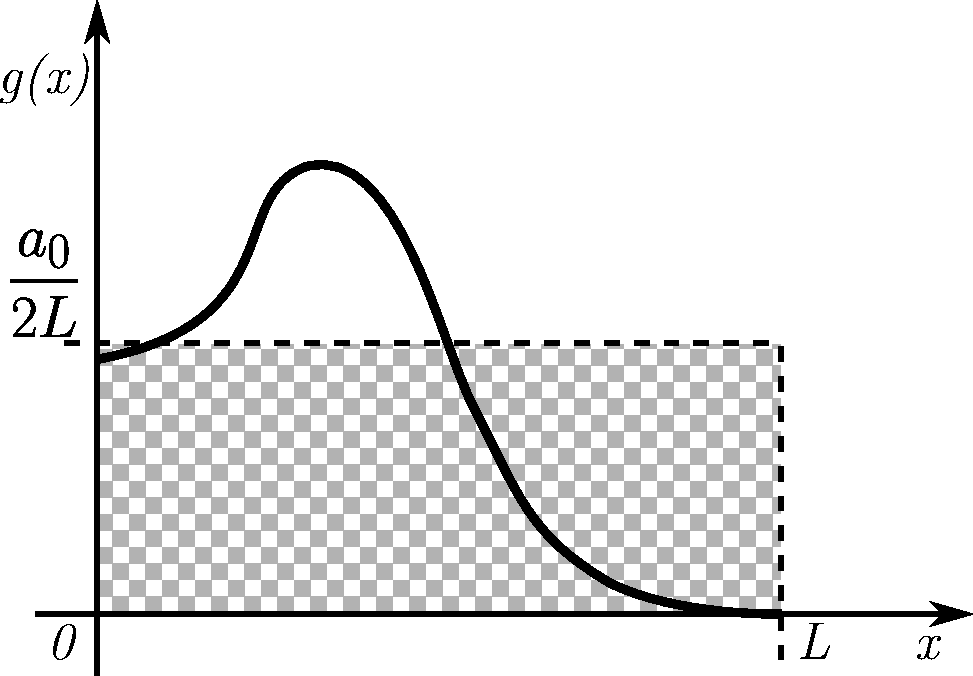
\includegraphics[width=0.5\textwidth]{isol_bar.pdf}
	\caption{Valor medio di $g(x)$ con barra isolata}
	\label{isol_bar}
\end{figure}

